This section describes the image processing pipeline that is delivered with the system and that has yielded the best performance so far. Some less successful attempts are described in appendices \ref{sec:bg_subtraction}, \ref{sec:hough_circles}, and \ref{sec:stereoBM}. 

\subsection{Sensors}
After reading several papers on counting people using a single camera with top-down view, and implementing the methods described in said papers, the realization was made that, in order to be able to solve the problem described in section \ref{sec:introduction}, some form of depth information would be necessary. Both stereo and Kinect-style sensors were considered. However due to time limitations and a customer desire to run the system on cheap hardware, the Microsoft Kinect sensor was chosen.

\subsection{Image processing}
The human segmentation is based on the assumption that human heads are distinguishable modes in the depth image and that people moving very close to each other seldom differ much more than a head in height. It is realized by a series of threshold and morphological operations, contour drawing and searches for local maxima. The output from some of the steps in the segmentation algorithm can be seen in figure \ref{fig:image_processing_steps}.

\begin{figure}[htb]
	\centering
	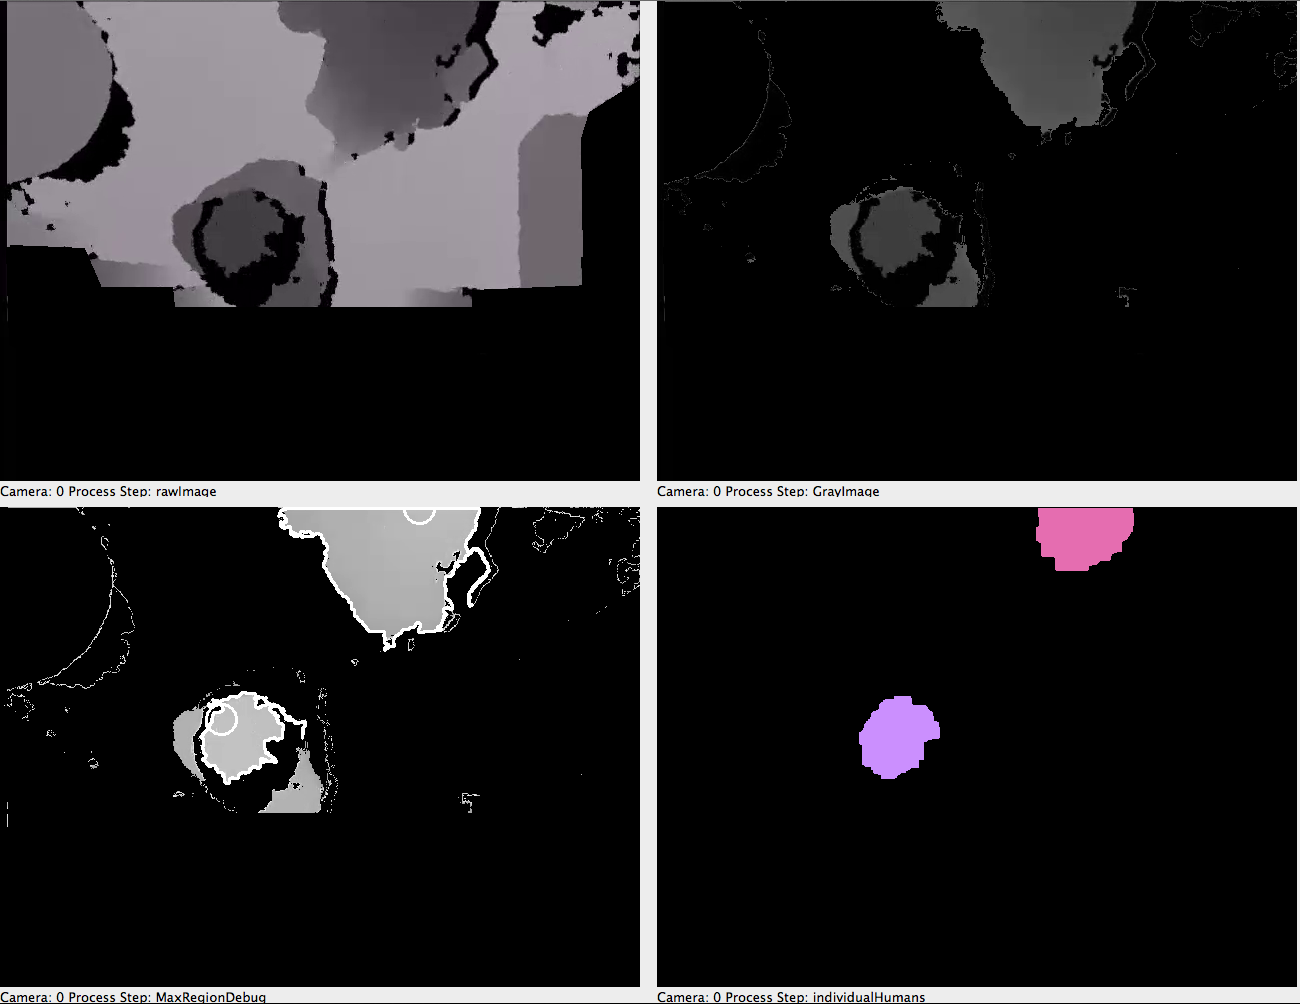
\includegraphics[width=\linewidth]{images/image_processing_steps.png}
	\caption[Image processing steps]{\textit{Image processing steps. The figure shows the results from four of the processing steps in the image processing pipeline.\\
		Top left: Raw depth image.\\ 
		Top right: Image after first threshold operation.\\ 
		Bottom left: Contour drawing and local maxima detection.\\ 
		Bottom right: Segmented human heads.}}
	\label{fig:image_processing_steps}  %Skapar referens till figuren
\end{figure}

\newpage
\subsection{Tracking and counting}
The tracking algorithm performs six different steps for each frame iteration. The tracker has a list objects found by earlier image processing steps and one list of objects passed from the previous frame. Tracking is done by pairing closest objects with each other, from previous frame to the current frame. Objects need to live for a predetermine configurable amount of frames before it will be counted. This prevent false flickering objects from generating false entries. Lost objects are also kept alive for some frames, this enables objects to be lost and found. Figure \ref{fig:trackingexample} illustrates how objects are seen as real objects, lost objects or potential objects, depending on their lifetime. 

\begin{figure}[htb]
	\centering
	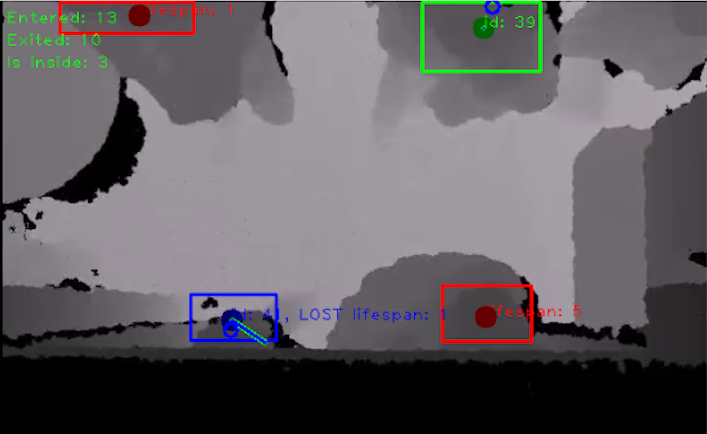
\includegraphics[width=0.7\linewidth]{images/trackingexample2.png}
	\caption[Tracking visualization]{\textit{Visualization of the tracking. The image shows one person (green box) who has lived long enough to be considered a person, two (red boxes) who has just been found and one (blue box) which is a person who’s just been lost}}
	\label{fig:trackingexample}  %Skapar referens till figuren
\end{figure}


To register if objects enter or exit the room the objects has to fulfill some requirements. To be considered as entered, an object has to be found in a door area and pass three circle lines in addition to have existed a minimum of a set amount of frames. To be registered as exited an object has to have existed a minimum of a set amount of frames and disappear inside a door area, while also at least once passed the three lines. Examples of these circle lines and a door area can be seen in figure \ref{fig:entry_exit}.

\begin{figure}[htb]
	\centering
	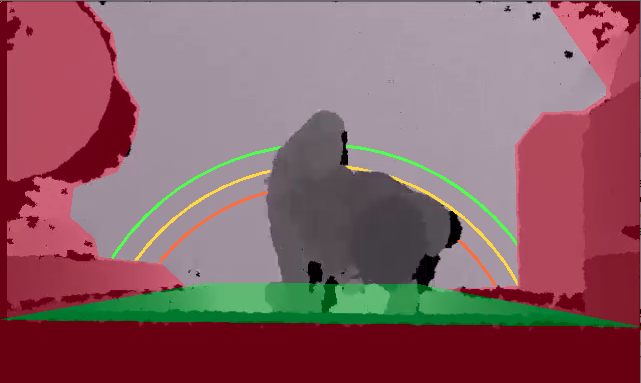
\includegraphics[width=0.7\linewidth]{images/entryexitexample.png}
	\caption[Checkpoint circles]{\textit{Entry and exit counting. Three circles are used to decide when a person has entered. The green area is the door area and the red area is excluded by the system.}}
	\label{fig:entry_exit}  %Skapar referens till figuren
\end{figure}

\newpage

\subsection{Queue severity estimation}
Queues are detected by using the positions and velocities, which are calculated using a simple Kalman filter, of all visible persons. This information is used to draw splines between each of the visible persons. Two people are then considered to be in a queue if a short enough spline can be drawn between them. The result is that persons that stand still or move slowly along the same path are considered to be in a queue. Examples of this can be seen in \ref{fig:visible_queue} and \ref{fig:no_queue}.
\\ \\
Queue severity is estimated by considering the proportion of frames with visible queues, and optionally the amount of people inside the room, over a set time interval. 
\begin{figure}[H]
\centering
\begin{subfigure}{.5\textwidth}
  \centering
  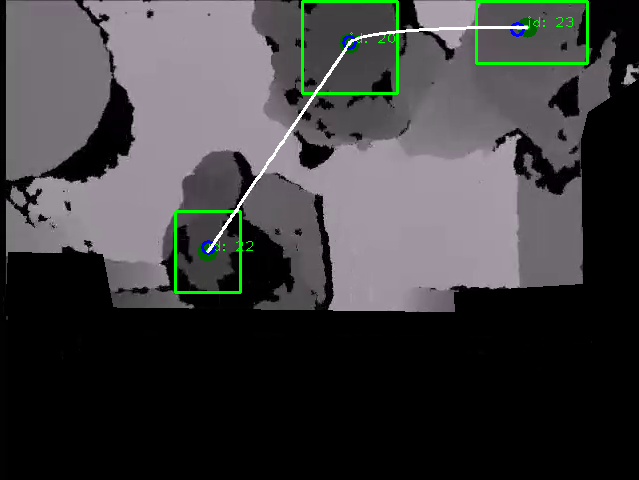
\includegraphics[width=0.9\linewidth]{images/visibleQueue.png}
  \caption{When persons are close together and moving slowly, \\
  			 they are connected by short splines and thus considered\\
  			  to be in a queue.}
  \label{fig:visible_queue}
\end{subfigure}%
\begin{subfigure}{.5\textwidth}
  \centering
  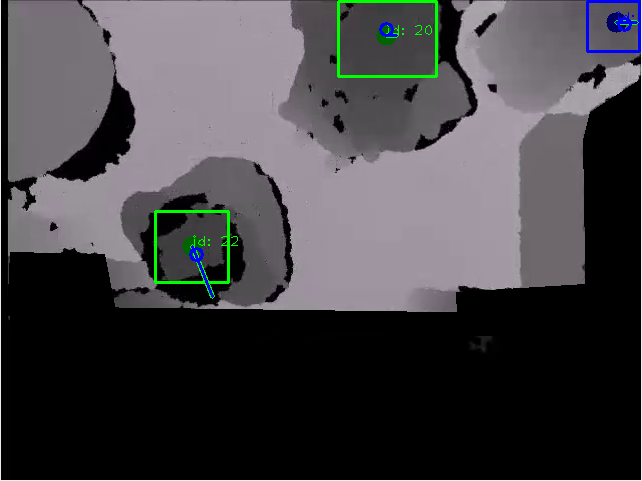
\includegraphics[width=0.9\linewidth]{images/noQueue.png}
  \caption{Persons moving in different directions, with large velocity, are connected by longer splines, and are thus not considered to be in a queue.}
  \label{fig:no_queue}
\end{subfigure}
\caption[Queue detection]{\textit{Detection of queues using splines. The images show the result of the queue detection steps in two different cases. Spines that are short enough are drawn to visualize detected queues.}}
\label{fig:queue_detection}
\end{figure}



